\solutionSection

Очевидно, что если $d > 2 \cdot r$, то за стол даже двух игроков не посадить и в качестве ответа нужно выводить $-1$. Далее будем решать задачу с дополнительным ограничением $d \le 2 \cdot r$.

Заметим, что при фиксированном количестве игроков, которых организаторы хотят усадить за стол, мы можем рассчитать наибольшую длину личного пространства, которое можно предоставить каждому из игроков.

Пусть организаторы хотят усадить за стол $n = 5$ игроков. Любым способом, который не противоречит условию, проведём хорды, отделяющие личное пространство игроков от остальной части стола (см. рис. 1).

Заметим, что могут остаться дуги, "не покрытые"\ ни одной из хорд. "Покроем"\ каждую из таких дуг одной из близлежащих хорд (см. рис. 2), что позволит не только не уменьшить длину наименьшего из предоставленных личных пространств, но и, возможно, увеличить эту длину.

Таким образом, получившиеся хорды стали образовывать $n$-угольник, около которого описана окружность.

\putImgWOCaption{16cm}{1st_tour/inf2/try_3/task_02/2019-04-09_065849.jpg}

%\begin{center}

%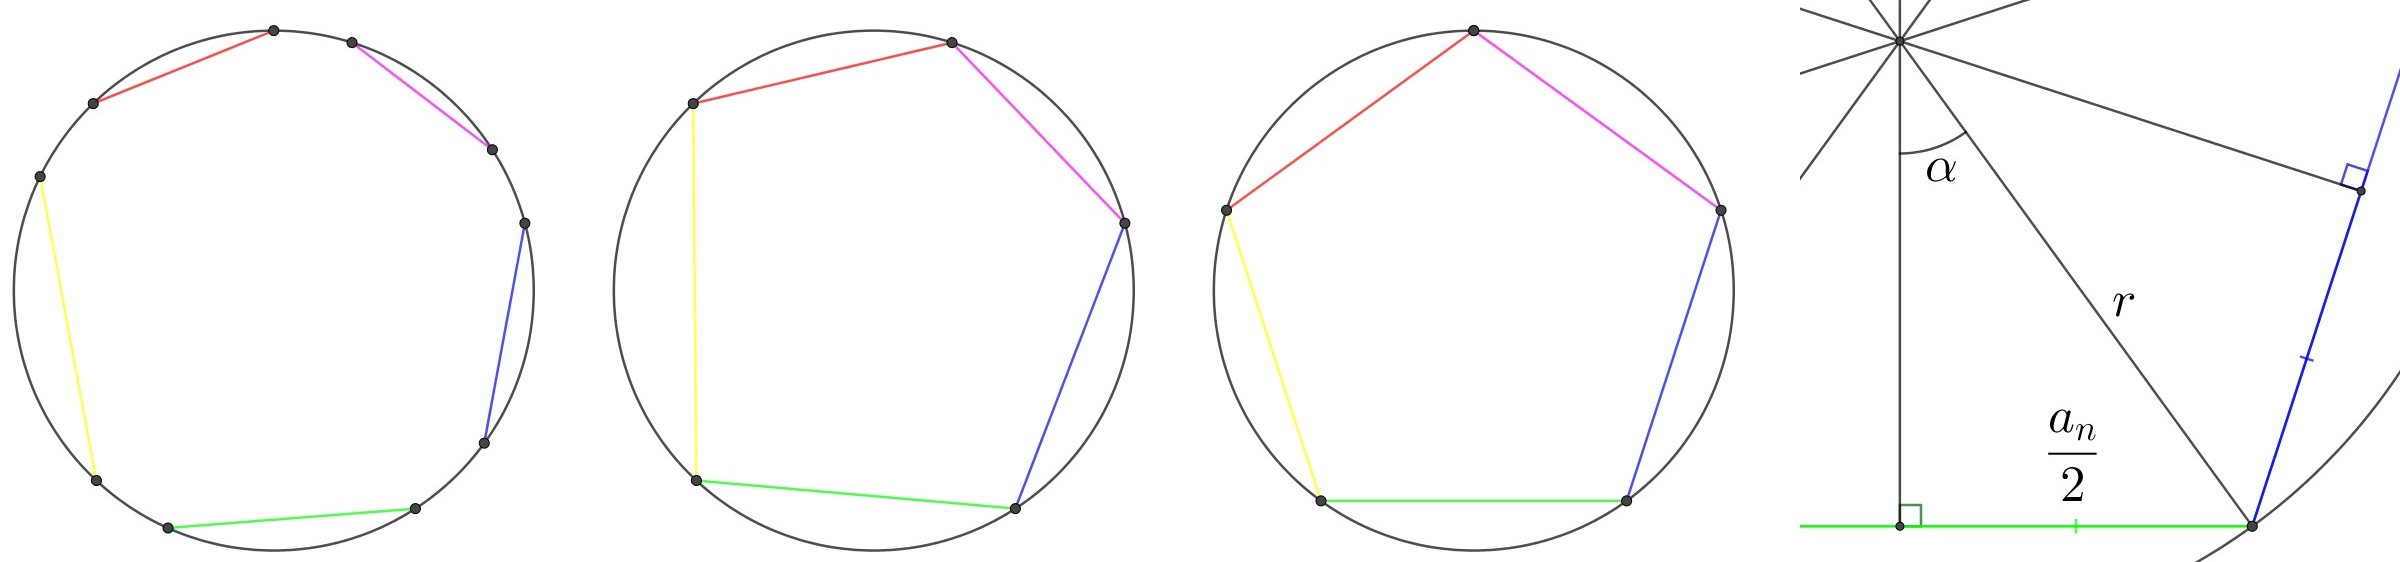
\includegraphics[bb = 460 20 100 130, scale = 0.75]{1st_tour_progr/task_032/2019-04-09_065849.jpg}

%\end{center}

Также заметим, что если существует пара хорд, длины которых различны, то длину меньшей из них можно увеличить за счёт уменьшения длины большей. 

А теперь заметим, что для максимизации длины личного пространства необходимо сделать все хорды равными по длине, поскольку если длина меньшей хорды не равна длине большей, то меньшую хорду можно увеличить за счёт большей, таким образом увеличив длину личного пространства.

В итоге хорды стали образовывать правильный $n$-угольник (см. рис. 3).

Используя свойства правильных многоугольников, можно вывести формулу, выражающую длину стороны правильного $n$-угольника через радиус описанной около $n$-угольника окружности (см. рис. 4):

\begin{center}

$\sin(\alpha) = \sin(\frac{2 \cdot \pi}{2 \cdot n}) = \frac{a_n}{2 \cdot r} \Leftrightarrow a_n = 2 \cdot r \cdot \sin(\frac{\pi}{n})$ , 

\end{center}

где $a_n$ -- длина стороны правильного $n$-угольника, которая в свою очередь равна наибольшей длине личного пространства, которое мы можем предоставить каждому из $n$ игроков на столе радиуса $r$.

Таким образом, остаётся определить ответ, который равен такому наибольшему $n$, что $a_n \ge d$. Искомое $n$ можно найти бинарным поиском по ответу, так как последовательность, заданная формулой $a_i = 2 \cdot r \cdot \sin(\frac{\pi}{i})$ для $i \ge 2$, является убывающей. Но можно пойти дальше и доказать, что ответом на задачу является $n = \left \lfloor \frac{\pi}{\arcsin(\frac{d}{2 \cdot r})} \right \rfloor$

\codeExample

%\inputPythonSource
%\inputJavaSource
\inputCPPSource